Introductory information theory with qubits.
\begin{parts}
	\part To examine entanglement, we first inspect the density matrices of the subsystems (Alice and Bob correspond to the left and right side of the notation):
	\begin{align*}
		\rho &= |a|^2 \ket{0+}\bra{0+} \\
		&\phantom{=} + ab^* \ket{0+}\bra{1-} \\
		&\phantom{=} + ba^* \ket{1-}\bra{0+} \\
		&\phantom{=} + |b|^2 \ket{1-}\bra{1-}
	\end{align*}
	
	In Dirac notation, the trace operation is defined as: $\textnormal{tr}\ket{a}\bra{b} = \braket{b|a}$, thus we have:
	\begin{align*}
		\rho_\textnormal{A} &= \textnormal{tr}_\textnormal{B}\, \rho \\
		&= |a|^2 \braket{+|+} \ket{0}\bra{0} \;+\; ab^* \braket{+|-} \ket{0}\bra{1} \\
		&\qquad + ba^* \braket{-|+} \ket{1}\bra{0} \;+\; |b|^2 \braket{-|-} \ket{1}\bra{1} \\
		&= |a|^2 \ket{0}\bra{0}
		+ |b|^2 \ket{1}\bra{1} \\[1em]
		\rho_\textnormal{B} &= |a|^2 \ket{+}\bra{+}
		+ |b|^2 \ket{-}\bra{-} \textnormal{\hspace{1em}similarly}
	\end{align*}
	
	Now we see that both density matrices are simply mixed states for non-zero $a$ and $b$, so the system state has to be entangled.
	
	Alternatively, calculating the purity for $\rho_\textnormal{A}$ and $\rho_\textnormal{B}$ would also work.
	
	\part The density matrix for the system:
	\begin{equation*}
		\rho = \frac{1}{2} \ket{00}\bra{00} + \frac{1}{2} \ket{\Phi^+}\bra{\Phi^+}
	\end{equation*}
	where $\ket{\Phi^+} = (\ket{00} + \ket{11})/\sqrt{2}$ is a Bell basis state.
	
	In matrix form it is simply:
	\begin{equation*}
		\rho =
		\begin{pmatrix}
			\diagfrac{3}{4} & 0 & 0 & \diagfrac{1}{4} \\
			0 & 0 & 0 & 0 \\
			0 & 0 & 0 & 0 \\
			\diagfrac{1}{4} & 0 & 0 & \diagfrac{1}{4}
		\end{pmatrix}
	\end{equation*}
	
	Following the instruction of the question, we diagonalise the density matrix:
	\begin{gather*}
		\begin{vmatrix}
			\diagfrac{3}{4}-\lambda & 0 & 0 & \diagfrac{1}{4} \\
			0 & -\lambda & 0 & 0 \\
			0 & 0 & -\lambda & 0 \\
			\diagfrac{1}{4} & 0 & 0 & \diagfrac{1}{4}-\lambda
		\end{vmatrix} = 0 \\
		\lambda^2 \left[\left(\frac{3}{4} - \lambda\right)\left(\frac{1}{4} - \lambda\right) - \left(\frac{1}{4}\right)^2\right] = 0 \\
		\begin{align*}
			\Rightarrow \lambda = 0 \textnormal{\hspace{1em}(Trivial root)} &
			\textnormal{\hspace{4em}or}&&\lambda^2 - \lambda + \frac{1}{8} = 0 && \\
			&&\lambda &= \frac{1 \pm \sqrt{1 - 4\times\diagfrac{1}{8}}}{2} && \\
			&& &= \frac{1 \pm \sqrt{\diagfrac{1}{2}}}{2} &&
		\end{align*}
	\end{gather*}
	
	Now recall the definition of von Neumann entropy:
	\begin{equation*}
		S = -\textnormal{tr}\left(\rho\log_2 \rho\right)
	\end{equation*}
	
	And further note that trace is basis invariant, therefore we have:
	\begin{align*}
		\rho\log_2 \rho &=
		\begin{aligned}[t]
			&\textnormal{diag}\left(0,\, 0,\, \frac{1+\sqrt{\diagfrac{1}{2}}}{2},\, \frac{1-\sqrt{\diagfrac{1}{2}}}{2}\right) \\
			&\cdot \textnormal{diag}\left(\log_2 0,\, \log_2 0,\, \log_2 \left(\frac{1+\sqrt{\diagfrac{1}{2}}}{2}\right),\, \log_2 \left(\frac{1-\sqrt{\diagfrac{1}{2}}}{2}\right)\right)
		\end{aligned} \\
		&= \textnormal{diag}\left(0,\, 0,\, -0.195,\, -0.406\right)
	\end{align*}
	Hence $S(\textnormal{AB}) = 0.601$.
	
	\part Perform partial trace on the system to get the density matrix for each side.
	By symmetry we simply consider one side:
	\begin{align*}
		\rho_\textnormal{A} &=
		\begin{pmatrix}
			\textnormal{tr}\begin{pmatrix}
				\diagfrac{3}{4} & 0 \\
				0 & 0
			\end{pmatrix} & 
			\textnormal{tr}\begin{pmatrix}
				0 & \diagfrac{1}{4} \\
				0 & 0
			\end{pmatrix} \\[1em]
			\textnormal{tr}\begin{pmatrix}
				0 & 0 \\
				\diagfrac{1}{4} & 0
			\end{pmatrix} &
			\textnormal{tr}\begin{pmatrix}
				0 & 0 \\
				0 & \diagfrac{1}{4}
			\end{pmatrix}
		\end{pmatrix} \\
		&=
		\begin{pmatrix}
			\diagfrac{3}{4} & 0 \\
			0 & \diagfrac{1}{4}
		\end{pmatrix}
	\end{align*}
	
	We then have the entropy for each of the subsystem as:
	\begin{align*}
		S(\textnormal{A}) = S(\textnormal{B}) &= -\textnormal{tr}\left[  \textnormal{diag}\left(\diagfrac{3}{4},\, \diagfrac{1}{4}\right) \cdot \textnormal{diag}\left(\log_2 \left( \diagfrac{3}{4}\right),\, \log_2 \left(\diagfrac{1}{4}\right)\right) \right] \\
		&= -\textnormal{tr}\left[ \textnormal{diag}\left(-0.311,\, -0.5\right) \right] \\
		&= 0.811
	\end{align*}
	
	\part As per the definition of mutual information, we have:
	\begin{align*}
		I(\textnormal{A}:\textnormal{B}) &= S(\textnormal{A}) + S(\textnormal{B}) - S(\textnormal{AB}) \\
		&= 1.022
	\end{align*}
	
	\part From part c, we have
	\begin{equation}
		\rho_\textnormal{A} = \frac{3}{4} \ket{0}\bra{0} + \frac{1}{4} \ket{1}\bra{1}
		\label{eqn:q6-rho-a}
	\end{equation}
	
	Rewriting \eqref{eqn:q6-rho-a} in the basis $\ket{\pm} = (\ket{0} \pm \ket{1})/\sqrt{2}$ gives:
	\begin{align*}
		\rho_\textnormal{A} &= \frac{3}{8} \Bigl(\ket{+}\bra{+} \;+\; \ket{+}\bra{-} \;+\; \ket{-}\bra{+} \;+\; \ket{-}\bra{-}\Bigr) \\
		&\qquad + \frac{1}{8} \Bigl(\ket{+}\bra{+} \;-\; \ket{+}\bra{-} \;-\; \ket{-}\bra{+} \;+\; \ket{-}\bra{-}\Bigr) \\[1ex]
		&= \frac{1}{2} \ket{+}\bra{+} \;+\; \frac{1}{4} \ket{+}\bra{-} \;+\; \frac{1}{4} \ket{-}\bra{+} \;+\; \frac{1}{2} \ket{-}\bra{-}
	\end{align*}
	From this we can immediately read that the probability of either outcome is $\diagfrac{1}{2}$.
	
	Alternatively we may think of the mixed state above as a lucky draw:
	\begin{figure}[H]
		\centering
		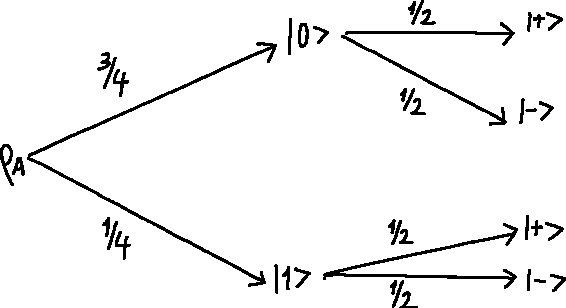
\includegraphics[width=.6\linewidth]{q6-tree-diagram}
	\end{figure}
	From the tree diagram, it is straightforward to see that the probability of each outcome is $\diagfrac{1}{2}$.
	
	However the very act of measurement has de-cohered Bob's qubit, hence the best description he has for his qubit would be:
	\begin{align*}
		\rho_\textnormal{B} &= \textnormal{diag}\left(\diagfrac{1}{2},\, \diagfrac{1}{2}\right) \\
		&= \frac{1}{2} \ket{0}\bra{0} + \frac{1}{2} \ket{1}\bra{1}
	\end{align*}
	
	\part The corresponding entropy for Bob's qubit would then be:
	\begin{align*}
		S(\textnormal{B}) &= -\textnormal{tr}\left[ \textnormal{diag}\left(\diagfrac{1}{2},\, \diagfrac{1}{2}\right) \cdot \textnormal{diag}\left(\log_2 \left(\diagfrac{1}{2}\right),\, \log_2 \left(\diagfrac{1}{2}\right)\right) \right] \\
		&= -\textnormal{tr}\left[ \textnormal{diag}\left(-0.5,\, -0.5\right) \right] \\
		&= 1
	\end{align*}
	
	Bob's entropy has increased as a result of the decoherence -- he no longer has any information on the state of his qubit!
\end{parts}